\chapter{Introduction}
\label{ch:introduction}

Progress in deep generative modelling is providing increasingly faithful models of real-world data. Deep generative models are now frequently used to generate images~\citep{rombach2022high,ho2022imagen} that are indistinguishable from photographs or the creations of visual artists. Generative models of language~\citep{wolf2020transformers} can generate long passages that pass as human-written. Generative models of molecules like proteins have been shown to generate novel yet feasible configurations that could revolutionise the process of drug discovery~\citep{hoogeboom2022equivariant,watson2022broadly}. 

A lot of real-world impact has come from \textit{conditional} generative models. 
One example application is as a tool for illustrators, enabling them to input a descriptive text caption and receive an image that fits this caption~\citep{rombach2022high,ho2022imagen}. Text-conditional video models serve a similar role for the quick generation or prototyping of videos~\citep{ho2022video}. In an image-editing use-case, a generative model will, at the very least, need to be conditioned on the image we wish to edit~\citep{rombach2022high,sheynin2023emu}. Large language models have achieved popularity when packaged as chat bots~\citep{wolf2020transformers} that generate responses conditioned on a user's prompts. If we want to generate plausible new drugs, we may wish to sample molecular structures conditioned on them having certain properties or interacting with target molecules~\citep{watson2022broadly}. Conditional generative models can also be used as ``digital twins'' simulating a piece of machinery, e.g. a jet engine, in silico~\citep{munk2022probabilistic,fuller2020digital}. Adjusting a digital twin's conditioning inputs allows the user to, e.g., predict the effect of tuning the settings of the jet engine. Weather forecasts with state-of-the-art accuracy can be obtained by conditioning models of atmospheric dynamics on up-to-date measurements~\citep{lam2022graphcast}. Conditioning generative models of text on input audio yields a state-of-the-art speech-to-text, or transcription, system~\citep{radford2023robust} and, similarly, conditioning generative models of audio on text yields state-of-the-art text-to-speech systems~\citep{tan2024naturalspeech}.


Many of the conditional generative models in these examples were trained from scratch, which takes significant time and expense; the compute costs for some recent training runs have been estimated at roughly 100 million US dollars~\citep{knight2023openai,stanford2024artificial}. One alternative to training from scratch is to derive a conditional generative model by modifying a previously-trained unconditional model~\citep{tian2023control,sheynin2023emu}. For example, simply using gradient descent to fine-tune the unconditional model's weights can lead to good performance. Other techniques like low-rank adaptation~\citep{hu2021lora}, which learns a low-rank modification of the pretrained model's weights, can further improve on this by reducing computational requirements and sometimes improving the quality of the resulting conditional model. Keeping the original weights frozen while adding additional network modules can similarly enable the fast training of conditional models~\citep{ruckle2020adapterdrop,tian2023control}.

% Doing so reduces the training cost and data requirements relative to training from scratch and is usually an acceptable solution if the number of conditioning tasks of interest, and therefore conditional models which must be finetuned, is limited.

When a lot of conditional generation tasks are of interest, however, performing any kind of task-specific optimisation may be too expensive. For example, for image inpainting, the ``task'' may be to condition on any conceivable subset of image pixels and so the number of possible tasks scales exponentially with the number of pixels. This leads to our interest in ``flexibly-conditional'' generative models that are designed to take as input a specification of what is conditioned on and then perform any of these conditional generation tasks without further training~\citep{ivanov2018variational,rombach2022high,zhao2021large,harvey2021conditional}. To be more precise, assume that we have data of fixed dimensionality $d$ which we denote $\rvx \in \mathbb{R}^d$. Some components of the data may be observed, where we define a component to be, e.g., a pixel if $\rvx$ is an image or a frame if $\rvx$ is a video. Let $\gY$ be a list of the indices of these observed components, and let $\rvy := \rvx[\gY]$ be their observed values. A flexibly-conditional generative model is one that can, at test-time, sample $\rvx$ given $\rvy$ and $\gY$ for any choices of $\rvy$ and $\gY$.


\begin{figure}
    \centering
    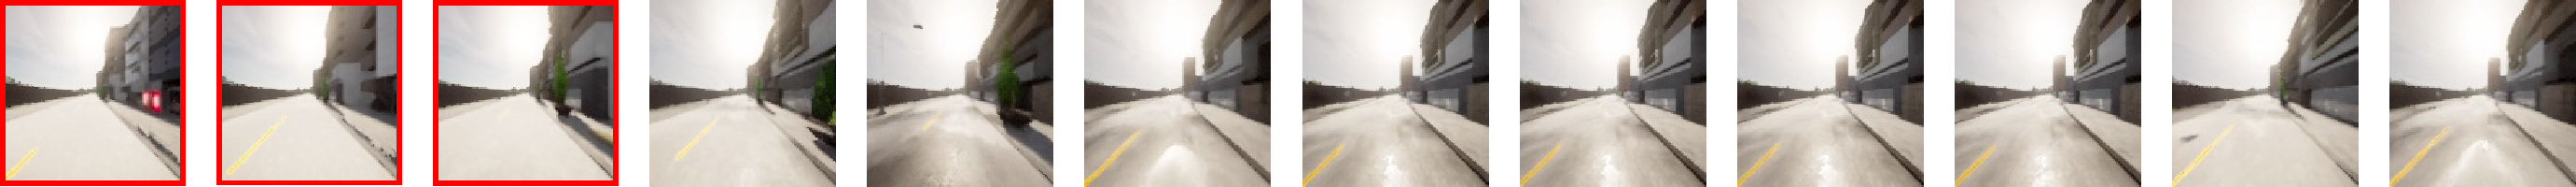
\includegraphics[width=\textwidth]{figs/thesis/fdm-example-tasks/world-modeling-thesis.pdf}
    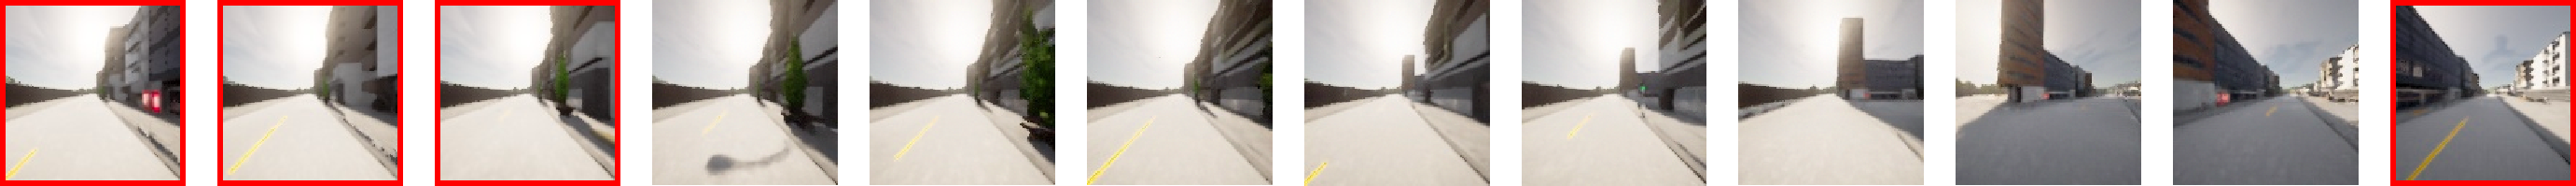
\includegraphics[width=\textwidth]{figs/thesis/fdm-example-tasks/visual-planning-thesis.pdf}
    \caption{Sampled 11-frame videos from a flexibly-conditional generative model that was trained on first-person data collected by a simulated autonomous vehicle within one virtual town. \textbf{Top:} A sample conditioned on the first three frames. This can be interpreted as conditioning on the vehicle's current state and predicting what it will do and see in the future. \textbf{Bottom:} A sample conditioned on a final ``goal'' frame as well as the first three frames. Conditioning on both the current state and a goal corresponds to goal-directed planning. }
    \label{fig:intro-world-modeling-and-planning}
\end{figure}

% The specific set of conditioning tasks that we may care about is domain dependent, but a reasonable goal in domains with data of fixed-dimensionality $d$ is to be able to generate data $\rvx \in \mathbb{R}^d$ conditioned on specified values of any arbitrary set of components of $\rvx$, where a component may be, e.g., a pixel if $\rvx$ is an image or, e.g., a frame if $\rvx$ is a video. To be more precise,
% % Denoting the data $\rvx \in \mathbb{R}^d$, a flexible generative model for this domain could ideally, at test-time,
% let us use $\gY$ to refer to a list of the indices of all observed components of a particular datapoint and use $\rvy := \rvx[\gY]$ to refer to the corresponding observed values. Then we define a flexible generative model as one that can approximate $\pdata(\rvx|\rvy,\gY)$ well for any given $\gY$ and $\rvy$, without retraining. This type of flexible model could enable many new use-cases in the domains described previously. Flexible models are already widely used in image editing, in the form of image inpainting models that can be conditioned on the values of any set of image pixels and then generate plausible values for the remainder~\citep{rombach2022high,zhao2021large,harvey2021conditional}.

\Cref{fig:intro-world-modeling-and-planning} hints at the tasks that such a flexibly-conditional model would be capable of in the video domain. If the video data is from the first-person perspective of an agent, having a flexibly-conditional model makes it possible to condition on previous frames as a representation of the agent's current or past state. We can additionally condition on near-future goals (e.g. desired locations) for planning tasks. Using the techniques we will introduce in this thesis, we can even condition on goals hundreds of frames in the future. In a reinforcement learning sense, this generative model is capable of doing any and all of: serving as a world model; implicitly modelling the agent's policy; and performing goal-directed planning. Future applications could include alternatives to (or integrations with) GPS-based navigation that can better incorporate visual cues in their planning, or controllers for advanced robots that take a visual input. One can similarly imagine a myriad of potential applications of flexibly-conditional generative models for, e.g., digital twins or in speech-to-text-style systems, but we limit the scope of this dissertation to the vision domain.

We point out two potential issues with the ``goal-directed planning'' application suggested above. The first is that, for it to be useful, we are likely to need our model to be capable of operating on very long videos with hundreds or thousands of frames. Video diffusion models are a state-of-the-art approach to video generation~\citep{ho2022video,blattmann2023align,brooks2024video} and are in principle amenable to flexibly-conditional generation using test-time guidance methods~\citep{ho2022video}. However, they can usually only operate on far fewer frames due to memory constraints. The models presented by \citet{ho2022video} jointly diffuse over at most 16 frames; the models presented by \citet{blattmann2023align} diffuse over at most 10 frames. Standard approaches to apply such models for the generation of longer videos, such as autoregressive roll-outs, are not compatible with flexibly-conditional generation. The second issue we raise is that, when specifying the goal frame in \cref{fig:intro-world-modeling-and-planning}, we had to know how much time it would take to reach. If we had a goal frame but did not know how long it would take to reach, we would not know the frame index we should condition on reaching the goal frame at. Ideally, we would be able to condition on reaching a frame ``at some point in the future'' without specifying a precise index.

The first two technical contributions we present make flexibly-conditional diffusion models robust to exactly these two issues. Our third core contribution is a method to speed up the training time of flexibly-conditional variational auto-encoders. More precisely:
\begin{itemize}
    \item In \cref{ch:fdm} we introduce a flexibly-conditional model of long videos. To enable flexibly-conditional generation of long videos with a diffusion model that can operate on relatively few frames at a time, we design the diffusion model to be able to generate values for any user-specified subset of frames conditioned on the values of any other user-specified subset. This allows us to optimise the order in which frames are generated at test-time, depending on what is most appropriate given the information to condition on. This contribution enables flexibly-conditional generation of long videos in addition to improved video quality in some settings.
    \item In \cref{ch:tddm} we present a diffusion model that is trained on data of varying dimensionality and which jointly samples the dimensionality of data points (such as the number of frames in a video) along with their values. When we apply test-time guidance, the values conditioned on naturally affect the dimensionality of the generated data as appropriate. This enables improved flexibly-conditional generation of data with unknown dimensionality.
    \item In \cref{ch:cigcvae} we tackle another barrier to the use of flexibly-conditional generative modelling: slow training times. We do so by introducing a simple technique to initialise a flexibly-conditional image generative model with the weights of an unconditional generative model. This was the first published method to do so within the variational auto-encoder framework and the resulting models outperformed all baselines at the time in terms of their representation of uncertainty given the conditioning signal.
\end{itemize}
Our contributions build heavily on the diffusion modelling framework~\citep{sohl2015deep,ho2020denoising}. Therefore, before describing them further, we will present background material on diffusion models in \cref{ch:diffusion}; on conditional diffusion models in \cref{ch:conditional-diffusion}; and on flexibly-conditional diffusion models in \cref{ch:flexible-diffusion}.


% We aim to demonstrate that generative models within the vision domain can be made flexible while retaining good performance, and sometimes with improved performance over our non-flexible baselines. 

% We will focus on demonstrating this within the diffusion modelling framework, which has become dominant for models of images and video~\citep{sohl2015deep,ho2020denoising,dhariwal2021diffusion,rombach2022high,ho2022imagen,peebles2022scalable,brooks2024video}. 

% We will therefore begin this thesis by reviewing the diffusion modelling framework in \cref{ch:diffusion}. We will show that diffusion models are naturally amenable to being used for conditional generation and even flexibly conditional generation of the type that we target in \cref{ch:conditional-diffusion,ch:flexible-diffusion}. 

% Our central contribution will be introducing innovations that enable flexible conditioning in challenging settings. 

% First we consider the long video domain where the complexity and dimensionality of typical datapoints is such that it is infeasible to take the standard approach of training a single model of all frames in \cref{ch:fdm}. Next we will target flexible generative modelling in domains where the dimensionality of different data points varies and so must be sampled along with the data values given any conditioning information in \cref{ch:tddm}; this is challenging for traditional conditional generative models. Finally, we recognise that the diffusion modelling may not remain the dominant paradigm for generative modelling of images and video forever. We therefore end by demonstrating that a different generative model class, that of variational auto-encoders, is also amenable to being used to build flexible generative models in \cref{ch:cigcvae}.
